\documentclass[11pt, oneside]{article}   	% use "amsart" instead of "article" for AMSLaTeX format
\usepackage{geometry}                		% See geometry.pdf to learn the layout options. There are lots.
\geometry{letterpaper}                   		% ... or a4paper or a5paper or ... 
%\geometry{landscape}                		% Activate for rotated page geometry
%\usepackage[parfill]{parskip}    		% Activate to begin paragraphs with an empty line rather than an indent
\usepackage{graphicx}				% Use pdf, png, jpg, or eps§ with pdflatex; use eps in DVI mode
								% TeX will automatically convert eps --> pdf in pdflatex		
\usepackage{amssymb,amsmath}
\usepackage{natbib,verbatim}
\usepackage{hyperref}
\usepackage{aas_macros}

\usepackage{changes}
\definechangesauthor[name=AK, color=blue]{1}
\definechangesauthor[name=EL, color=red]{2}

\title{LBL Peculiar-Velocity Program}
\author{Greg Aldering, Alex Kim, Peter Nugent, Saul Perlmutter}
%\date{}							% Activate to display a given date or no date

\begin{document}
\maketitle


%\section{}
%\subsection{}
Measuring peculiar velocities using Type~Ia supernovae is a primary research topic in the upcoming decade.  Peculiar velocities have
been cited as a part of the   Small Projects Portfolio  by the the Cosmic Visions Dark Energy Working Group \citep{2018arXiv180207216D}.
This document presents a range of programs that the LBL SN scientists would like to pursue including established surveys such as ZTF, ZTF-II,
DESI, LSST, and new but complementary initiatives.

\section{Probing Gravity With SN~Ia  Peculiar Velocity Surveys}
In the late 1990's, Type~Ia supernovae (SNe~Ia) were used as distance probes to measure the homogeneous expansion history of the Universe.  The remarkable discovery
that the expansion is accelerating  has called into question our basic understanding of the gravitational forces within the Universe.  Either it
is dominated by a ``dark energy'' that is gravitationally repulsive, or General Relativity is inadequate and needs to be replaced by a modified theory of
gravity.  It is only appropriate that in the upcoming decade, with their sheer numbers, solid-angle coverage,
and improved distance precisions, SNe~Ia will provide measurements of the {\it inhomogeneous} motions of structures in the Universe
that will provide an unmatched test of whether dark energy or modified gravity is responsible for the accelerating expansion of the Universe.

In the next decade, SNe~Ia will be used as peculiar-velocity probes to measure  the influence of gravity on structure formation within the Universe.
Peculiar velocities induce scatter along the redshift axis of the SN Hubble diagram, which is
pronounced at low redshifts and when the magnitude scatter (e.g.\ due to intrinsic magnitude dispersion) is small.
The conservation of mass relates peculiar velocities  with mass overdensities in the same volume through the continuity equation
$Haf\delta(\mathbf{x}) + \nabla \cdot \mathbf{v}(\mathbf{x}) =0$ where the linear growth rate $f \equiv \frac{d\ln{D}}{d\ln{a}}$, $a$ is the scale factor, and $D$ is  the spatially-independent
``growth factor''.
Though the fields are not directly comparable, the power spectra in different volumes are such that
the peculiar velocity power spectrum and the overdensity power spectrum at the surface of last scattering are related by
$P_{vv}\propto (fD)^2P_{\delta \delta}(z_{\text{CMB}})$  \citep{2006PhRvD..73l3526H,2011ApJ...741...67D}. 
The $\Lambda$CDM prediction for the $z=0$ peculiar velocity power spectrum given CMB data is shown in Figure~\ref{power:fig}.


\begin{figure}
\centering
\includegraphics[width=0.6\textwidth]{/Users/akim/project/PeculiarVelocity/doc/src/new2.png}
%\includegraphics[width=0.5\textwidth]{../outcosmo/zmax_.png}
\caption{Dimensionless peculiar velocity power spectrum $k^3P_{vv}(z=0)$ for $\mu \equiv \cos{(\hat{k} \cdot \hat{r})}=1, 0.5$ (magenta, cyan) 
where $\hat{r}$ is the line of sight, as predicted for General Relativity in the linear regime.
Overplotted are peculiar-velocity power-spectrum shot noise  (diagonal lines) for various observing parameters.  Red shows the shot noise expected from a 2-year LSST survey
while black shows a 10-year LSST survey.  The dotted and dashed lines indicate the assumed intrinsic magnitude dispersion, using 0.08 (dashed) or 0.15 mag (dotted).  The expected shot
noise from TAIPAN is shown in green (dash-dotted). 
%
%Overplotted are volume-weighted peculiar velocity shot-noise  $k^3\sigma^2/n$ at $z=0.1$ expected from 2- and 10-year (red, black) supernova densities, 0.08 and 0.15~mag (dashed, dotted) intrinsic magnitude dispersions, and TAIPAN (green, dash-dotted).
The bottom solid grey horizontal lines show the approximate range of $k$ expected to be used in surveys with corresponding
redshift depths $z_{\rm max}$.
\label{power:fig}}
\end{figure}


%The bias is a ``nuisance'' parameter, not present in the velocity power spectrum, which must marginalized out when inferring $\gamma$.
%The same field is responsible for both overdensities and velocities so when combined in a common analysis the sample variance limit is lowered.

Galaxy surveys complement peculiar-velocity surveys.  As alluded to earlier,
comparing a peculiar velocity survey with an overlapping galaxy survey provides a measure of $f/b$, where $b$ is the galaxy bias.
In addition, Redshift Space Distortions in the galaxy survey measure growth through  $P_{\delta \delta }\propto (bD + fD\mu^2)^2P_{\delta \delta}(z_{\text{CMB}})$,
where $\mu\equiv \cos{(\hat{k} \cdot \hat{r})}$ where $\hat{r}$ is the direction of
the line of sight.
A single SN~Ia peculiar-velocity survey, whose SN search maps SN overdensities, thus gives three measures of growth, though the large number density
of galaxies relative to decades worth of SNe means that better constraints are possible using an independent galaxy survey.

The  growth of structure depends on gravity;
\citet{PhysRevD.72.043529,2007APh....28..481L} find that General Relativity, $f(R)$,  and DGP gravity follow the relation
$f \approx \Omega_M^\gamma$ with the growth index $\gamma=0.55, 0.42, 0.68$ respectively \citep[see][for a review
or these  models]{HUTERER201523}.  
Using this parameterization, peculiar velocity
surveys probe  gravity through by modeling $fD=\Omega_M^{\gamma} \exp{\left(-\int_a^1 \Omega_M^{\gamma} d\ln{a} \right)}$,
where $\Omega_M(a)$ also depends on the gravity model.
The  $\gamma$-dependence of $fD(z)$ is shown 
in Figure~2 of  \citet{1475-7516-2013-04-031}.

%
%The parameter $\sigma_8$, the  standard deviation of overdensities in 8$h^{-1}$Mpc spheres, is 
%commonly used in place of $D$ to normalize the
%overall amplitude of  overdensities, so the standard parameterization used by the community is $f\sigma_8$.}




A SN~Ia peculiar velocity survey is composed of several components:
\begin{itemize}
\item Transient Discoveries -- Wide-field cadenced imaging surveys detect and localize the angular coordinates of new supernovae.
\item Discovery Screening -- Galaxy redshift catalogs, supplemental imaging data can provide subsets of the discoveries for classification
using relatively expensive follow-up resources.
\item SN~Ia Classification -- Spectroscopy classifies the SN~Ia from among the pool of  transient discoveries. 
\item (Host-galaxy) Redshift -- Spectroscopy provides redshifts. 
Host-galaxies generally have more/sharper features that provide more precise redshifts than the supernovae themselves. Resolution $R>200$
is sufficient to ensure that statistical uncertainties are negligible.
\item SN~Ia Distance -- Imaging produces photometry and colors for light-curve fitting and getting distances.  The transient search naturally provides some data
for this, of quality that varies depending on the survey strategy.
Spectroscopy and NIR photometry
have been shown to provide more precise distances than with optical light curves alone.
\end{itemize}
The above suite of observations provide a pure sample of SNe~Ia with observed redshifts and cosmological redshifts (inferred from the distances and
the background Hubble law)
whose difference is the radial peculiar velocity.

The precision  in measuring $\gamma$ can be projected for different peculiar velocity surveys.
The primary  parameters that affect the precision are: solid angle $\Omega$, SN number density $n$, source intrinsic
magnitude dispersion $\sigma_M$, and for a distance-limited survey the maximum distance $r_{\text{max}}$ (alternatively redshift $z_{\text{max}}$).
The dependence is most simply discerned 
in the  Fisher information matrix
\begin{align}
F_{ij} 
%& = \frac{V}{2}\int \frac{d^3k}{(2\pi)^3} \text{Tr}\left[ C^{-1} \frac{\partial C}{\partial \lambda_i} C^{-1}
%\frac{\partial C}{\partial \lambda_j} \right]\\
& = \frac{\Omega}{8\pi^2} \int_{r_{\rm min}}^{r_{\rm max}}  \int_{k_{\rm min}}^{k_{\rm max}}  \int_{-1}^{1} r^2 k^2 \text{Tr}\left[ C^{-1} \frac{\partial C}{\partial \lambda_i} C^{-1}
\frac{\partial C}{\partial \lambda_j} \right] d\mu\,dk\,dr
\label{fisher:eqn}
\end{align}
where
\begin{equation}
C(k,\mu,a)  =
  \begin{bmatrix}
   P_{\delta \delta}(k,\mu,a) + \frac{1}{n} &
   P_{v\delta}(k,\mu,a)  \\
   P_{v\delta}(k,\mu,a)  &
  P_{vv}(k,\mu,a) + \frac{\sigma^2}{n}
   \end{bmatrix},
\label{cov:eq}
\end{equation}
and the
peculiar-velocity  uncertainty  ($\sigma$) is related to magnitude uncertainty via $\sigma_M^2 =  \left(\frac{5}{\ln{10}}\right)^2 \left(1-\frac{1}{Ha\chi}\right)^2 \sigma^2$.
The dependences of $\gamma$ and other parameters enter through $fD$ in the relations $P_{vv}\propto (fD\mu)^2$, the SN~Ia host-galaxy count overdensity
power spectrum $P_{\delta \delta }\propto (bD + fD\mu^2)^2$, and the galaxy-velocity cross-correlation $P_{vg}
\propto  (bD + fD\mu^2)fD\mu$.  
 The density and velocity covariances depend on the parameter set $\lambda \in \{\gamma, \Omega_{M0}, b\}$.
Taking $\Lambda$CDM as our fiducial model, 
$\Omega_M=\frac{\Omega_{M_0}}{\Omega_{M_0} + (1-\Omega_{M_0})a^3}$.  
The uncertainty in the growth index is bounded by $\sqrt{F^{-1}_{\gamma \gamma}}$.

\section{Current Results and Projections}
\subsection{Current Results}
Peculiar velocity surveys have already been  used to measure
the effective $fD$ in redshift bins  (referred to as $f\sigma_8$), though not to a level where  gravity models can be precisely distinguished.
 \citet{2017MNRAS.471..839A} use 6dFGS peculiar velocities using  Fundamental Plane distances of elliptical galaxies to estimate absolute magnitudes
 with
 $\sim 0.43$~mag  precision, yielding a 15\% uncertainty in $fD$ at $z\approx 0$.
The upcoming 
TAIPAN survey \citep{2017PASA...34...47D} will obtain Fundamental Plane galaxies with densities of $n_g \sim 10^{-3}h^3$\,Mpc$^{-3}$,
and the WALLABY+WNSHS surveys \citep{2008ExA....22..151J} will obtain Tully-Fisher distances (based on the $\sim 0.48$~mag calibration of absolute magnitude based on the  HI 21cm line width)
of galaxies with densities $n_g \sim 2\times 10^{-2} - 10^{-4} h^3$\,Mpc$^{-3}$ from
$z=0-0.1$ covering 75\% of the sky.
These surveys combined are projected to have 3\% uncertainties in $fD$ \citep{2017MNRAS.464.2517H}.
For reference, DESI projects a 10\% precision of $fD$ at $z \approx 0.3$  by looking 
for signatures (Redshift Space Distortions; RSD) expected from galaxies infalling toward mass overdensities.
Relative to galaxies with  Fundamental Plane or Tully-Fisher distances, 
SN~Ia host galaxies currently have significantly lower number density but have better per-object peculiar velocity precision.
Existing SN~Ia samples
have been used to test and ultimately find spatial correlations in peculiar velocities that may be attributed to the growth of structure
\citep{PhysRevLett.99.081301,2008MNRAS.389L..47A,2014MNRAS.444.3926J,2015JCAP...12..033H, 2017JCAP...05..015H}.
SNe~Ia discovered by ASAS-SN, ATLAS, and ZTF \citep{2014ApJ...788...48S,2018PASP..130f4505T,2019PASP..131a8002B} over the next several years will provide first probative measures of $fD$ at $z<0.1$.
%Measurement of the velocity field using LSST-discovered
%SNe~Ia has been quantified by \citep{2011PhRvD..83d3004B,2017JCAP...01..060O}

\subsection{Projections}
Two advances in the upcoming decade will make SN~Ia peculiar velocities more powerful.
First, the precision of SN~Ia distances can be improved.  The commonly-used empirical 2-parameter spectral model yields  absolute magnitude
dispersion $\sigma_M \gtrsim 0.12$~mag.  However, SNe transmit more information than just the light-curve shape and single color used in current SN models.
Recent studies indicate that with the right data, SN absolute
magnitudes can be calibrated to $\sigma_M \lesssim 0.08$ mag \citep[see e.g.][]{2012MNRAS.425.1007B, 2015ApJ...815...58F}. 
Though not yet
established, it is anticipated that such a reduction in intrinsic dispersion comes with a reduction in the magnitude bias correlated with host-galaxy properties
that is observed using current calibrations.  At this precision the intrinsic velocity dispersion  at $z=0.028$ is  $300$~km\,s$^{-1}$, i.e.\ a single SN~Ia  is of such quality as to
measure a peculiar velocity with $S/N \sim 1$.
 If corrections of all SNe~Ia are not possible, the use of SN~Ia subclasses is an option though at the expense of reducing the
numbers of velocity probes.
Secondly,  in the upcoming decade cadenced wide-field imaging surveys such as ZTF2 and LSST
  will increase the number of identified  $z<0.2$ Type~Ia supernovae from the hundreds to the
hundreds of thousands; over the course of 10-years, LSST will find $\sim150,000$ $z<0.2$ SNe~Ia
 for which good light curves can be measured, corresponding to a  number density of $n \sim 5\times 10^{-4}h^3$\,Mpc$^{-3}$.
  This sample has comparable
 number density and more galaxies at deeper redshifts than projected by WALLABY and TAIPAN.  With similar densities,
 the (two) ten-year SN~Ia survey will have
 a (6) 29$\times$ reduction in shot-noise, $\sigma^2_M/n$, relative to the Fundamental Plane survey of TAIPAN.

A SN~Ia peculiar velocity program hinges on  SN discoveries, the number density $n$ of which
depends on the cadenced wide-field imaging survey used for the search.    
It is thus convenient to make projections for upcoming programs
based on the imaging survey; the projections here use ZTF2 and LSST 
as canonical representatives.
Keep in mind that other follow-up resources determine the distance precision $\sigma_M$, the other important parameter
that affects projections.


The primary sources of systematic error in a high-redshift supernova Hubble diagram are not as important for a low-redshift
peculiar velocity survey.  A Hubble diagram that spans a broad redshift range requires absolute color calibration over the corresponding observer-frame
wavelength range and control over the different populations over the span of cosmic time from which SNe are drawn.  High-redshift peculiar
velocity measurements do not have much sensitivity to $\gamma$, and a SN survey confined to lower redshifts is less sensitive to
color-calibration uncertainties and population evolution.

Details on the assumptions made for the calculations that follow can be found in \citet{2019BAAS...51c.140K}.

\subsubsection{Near-Term: ZTF2}
ZTF2 and TAIPAN are near-term surveys that will measure peculiar velocities, the former using SNe~Ia and the latter
using Fundamental Plane Galaxies.  Both have roughly
 $z_{\text{max}}=0.09$ and $\Omega = 2\pi$.
Uncertainties in $\gamma$ for surveys with this depth and solid-angle coverage 
are shown as a function of number of sources $N$ and $\sigma_M$ in Figure~\ref{surface:fig}. 

The positions of ZTF2 and TAIPAN are marked
in the figure, with the former showing both  a conservative $\sigma_M=0.12$~mag and aggressive $\sigma_M=0.08$~mag.
The former is the uncertainty that could be achieved with ZTF2 photometry alone, the latter with additional
SN follow-up.
ZTF2 and TAIPAN lie in opposite ends of the figure, there are small numbers of ZTF2 SNe with precise distances
whereas there are many TAIPAN Fundamental Plane galaxies with imprecise distances. 
Conservative ZTF2 and TAIPAN
are projected to give similar precisions $\sigma_ \gamma = 0.060$, whereas  aggressive ZTF2 gives a more constraining
$\sigma_ \gamma = 0.048$.  
Recall that the difference in $\gamma$  between GR and the $f(R)$ and DGP gravity is 0.13, meaning that the surveys
can already distinguish between these models to $2-3 \sigma$.

\begin{figure}
\centering
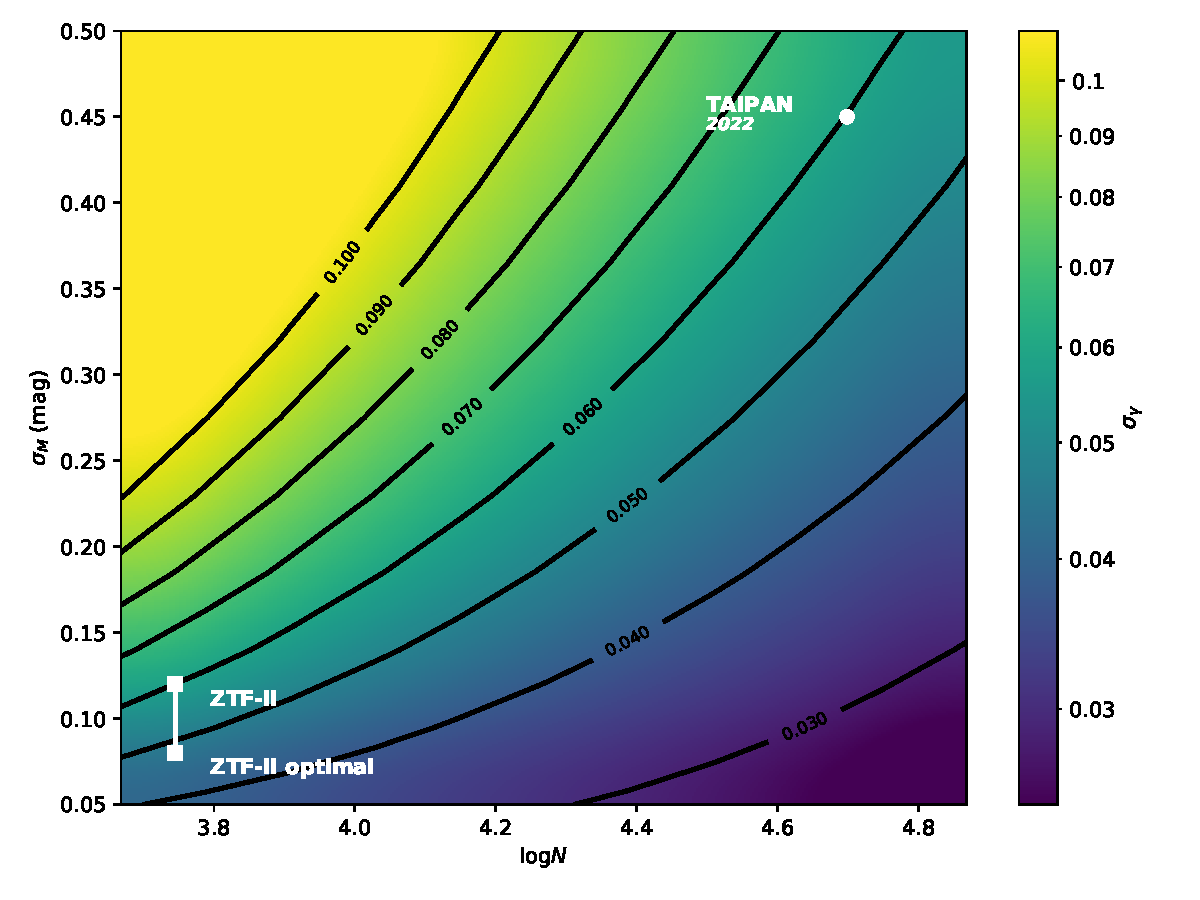
\includegraphics[width=0.6\textwidth]{src/surface1.pdf}
\caption{Uncertainties in $\gamma$ for surveys  with $z_{\text{max}}=0.09$ and $\Omega = 2\pi$
are shown as a function of number of sources $N$ and $\sigma_M$.  The positions of ZTF2 and TAIPAN are marked,
with the former showing both  a conservative $\sigma_M=0.12$~mag and an aggressive $\sigma_M=0.08$~mag.
\label{surface:fig}}
\end{figure}

An important distinction between the surveys is
that TAIPAN will observe almost all available Fundamental Plane galaxies in the local volume, meaning that no additional observing can
increase the number density $n$ and decrease $\sigma_\gamma$.  On the other hand, the number density of supernova increases
linearly with time, there is continued room for decreased $\sigma_\gamma$ with longer surveys  as ZTF2 is not  sample-variance limited 


ZTF2 and TAIPAN are not in competition but are complementary.  Being in different hemispheres, the two surveys
cover different parts of sky, meaning that their two independent results can be
combined  quadratically to produce a reduced joint uncertainty. 

\subsubsection{Long-Term: LSST}
A long-term supernova peculiar-velocity survey can be performed with SNe~Ia discovered by LSST.
As a 10-year survey, LSST generates higher supernova number densities to fainter limiting magnitude than  ZTF2,
making possible significantly improved constraints on the growth index.
All the proposed LSST surveys have complete SN~Ia discovery out to $z=0.3$.
The expected distance uncertainties derived from LSST light curves vary greatly depending on observing strategy, but at best
is expected to be $\sigma_M=0.12$~mag. Some strategies provide SN discovery but much poorer light curves
and distances.   As with the ZTF2 survey,  lower magnitude uncertainties
can be achieved with supplemental data.

Uncertainties in $\gamma$ for surveys with a 10-year duration   and $\Omega=2\pi$ sky coverage, applicable to the LSST WFD survey, 
are shown as a function of limiting  redshift $z_{max}$ and $\sigma_M$ in Figure~\ref{lsst:fig}.
The redshift depth afforded by LSST provides significant improvement relative to the shallower ZTF2 survey.
After 10 years, the region with $z_{max}<0.1$ has $\sigma_\gamma$ that is only weakly $\sigma_M$-dependent, 
which reflects the relatively strong sample variance in the small local survey volume.  
As $\sigma_\gamma$ quickly increases for surveys shallower than the $z_{\text{max}}=0.09$ 
of ZTF2,
better growth index constraints
are achieved by going to $z_{max}>0.1$.
The gradient in decreasing $\sigma_\gamma$ does shallow out with increasing redshift despite the increased survey volume, 
as the velocity uncertainties degrade with redshift for a fixed $\sigma_M$.

\begin{figure}
\centering
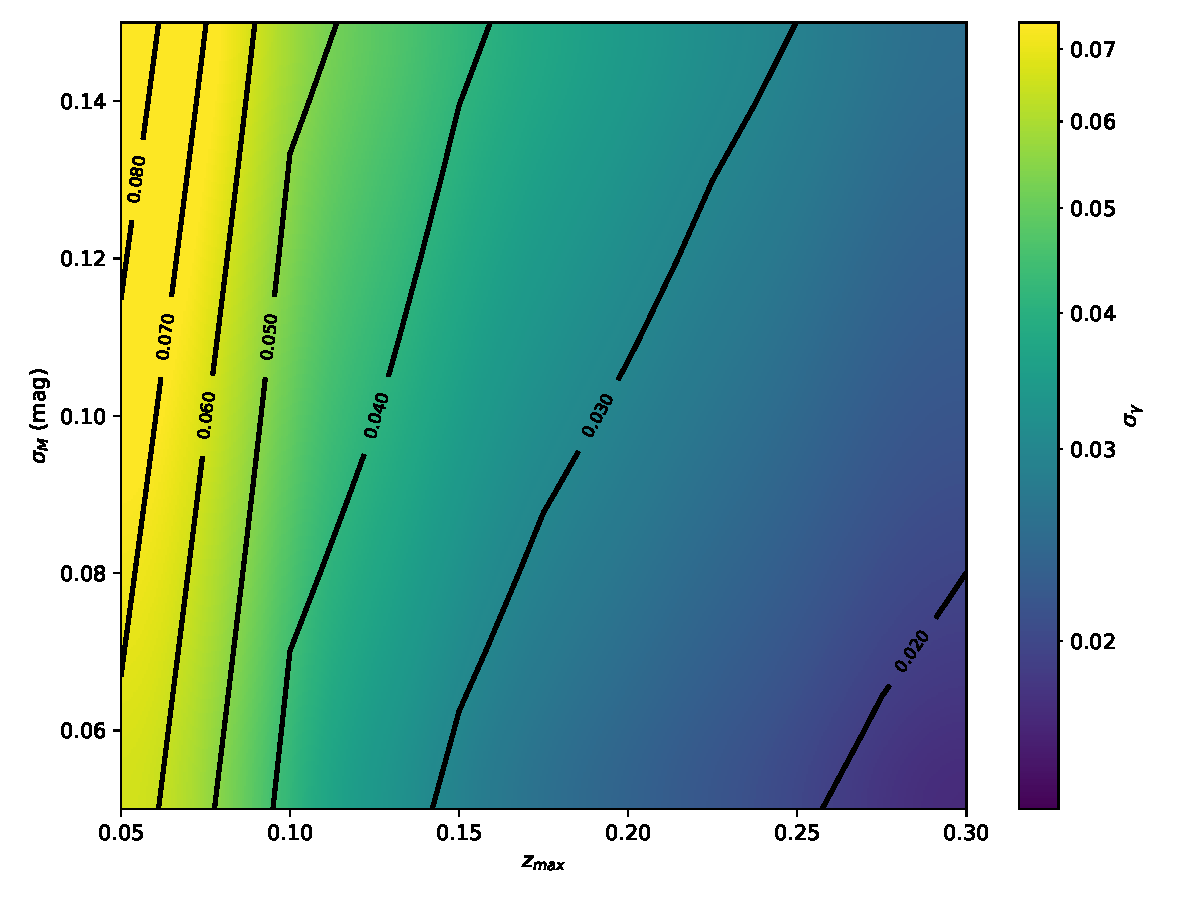
\includegraphics[width=0.6\textwidth]{src/surface2.pdf}
\caption{Uncertainties in $\gamma$ for surveys with a 10-year duration and  and $\Omega=2\pi$ sky coverage 
are shown as a function of limiting  redshift $z_{max}$ and $\sigma_M$.
\label{lsst:fig}}
\end{figure}

\subsection{Complementarity with High-$z$ redshift surveys}
Combined low-redshift peculiar velocity and high-redshift RSD $fD$ measurements (i.e.\ from DESI) are highly complementary as together they probe the
$\gamma$-dependent shape of $fD(z)$ (not just its normalization) and potential scale-dependent influence of gravitational models.  
The latter is true because 
the $k_{\text{max}}$ of linear modes for the RSD measurement is higher than that of the low-redshift peculiar velocity measurement.

\section{Plan for a Peculiar Velocity Program}
The projections for measuring $\gamma$ with ZTF2 and LSST SN~Ia discoveries
show the power of peculiar velocities surveys at low redshift.
This  tracer provides an unmatched  new window with which to test gravity and the source of the accelerating expansion of the Universe.
We propose the following course of research for the upcoming decade.

\subsection{Present}
The current goals are to provide a proof of concept of a SN peculiar velocity survey while developing domain
expertise and pipelines that can be used in future experiments.

Kim has developed a SNFactory/ZTF peculiar-velocity analysis framework with a postdoc.  Its distinguishing features is that it is likelihood-based
including both density and peculiar velocities.  The complexity of including fitting the underlying mass density field in the model
is addressed through Hamiltonian Monte Carlo.  Analytic expressions for the partial derivatives of the likelihood are coded,
avoiding the computational limitations of {\it autodiff} in STAN.  A end-to-end implementation is complete, validation of it is ongoing.

The first application o the analysis pipeline will be for SNFactory supernovae.  A next analysis will be of ZTF-discovered 
SNe when those data are ready.  The plan is for a  subset of the required data, precision redshifts of SN host galaxies, to be provided
by DESI.  Additional DESI data contributions are being discussed.

\subsection{Near Term: DESI as TAIPAN-North}

There has been talk of using BGS for a peculiar-velocity survey.  There is some question as to how deep the BGS achieves.  This should be
dug into.

\subsection{Near Term: ZTF2 + DESI}
A near-term peculiar velocity program can already provide the most competitive measurements of $\gamma$ at low redshift.  Engaging in science
now positions LBL for domain leadership in the LSST era.  For its near-term peculiar-velocity program, we advocate a survey using SN~Ia discoveries from ZTF2,
rather than other possible surveys, for the following reasons:
\begin{itemize}
\item A peculiar-velocity survey is already being touted as a primary science driver. As such,
the observing strategy should accommodate our needs.
\item It would be ready to start at the end of ZTF in 2021.
\item It is cheap, with a cost ranging from zero to access public data, to an amount (\$300k?) smaller
than building a new facility.
\item ZTF2 includes SEDMachine for classification of $m<18.5$~mag  transients.
\item It is in the Northern Hemisphere, which complements and is not superseded by LSST. 
Even after the nominal 3-year survey and simultaneous with LSST, the facility remains important for peculiar-velocity studies.
\item It is anticipated that the public plus private collaboration surveys can be designed to generate distance
precisions of $\sigma_M =0.12$~mag, which allow good velocity measurements with SNe~Ia.  (Additional follow-up can lower this uncertainty further.)
\item The limiting redshift $z_{\text{max}} =0.09$ is sufficiently deep  to have a scientifically interesting result $\sigma_\gamma < 0.053$.
There are other SN searches that do not achieve this depth.
\end{itemize}

ZTF2 SN~Ia discoveries are combined with data from other facilities to form a complete PV program.  We propose:
\begin{itemize}
\item DESI will provide the following components of the survey:
\begin{itemize}
\item Discovery Screening -- Provides redshifts for probable host galaxies of new transients, for use in early classification.  A host galaxy may
already have a DESI redshift, may be a BGS target without a redshift but whose observation could be prioritized,  or non-DESI target for which we
make a secondary-target fiber allocation.
\item SN Ia Classification -- Spectroscopy of active transients  through secondary-target fiber allocations within
DESI survey pointings. There
will be $\sim 1$ active $r<21.5$ SN~Ia in every three DESI pointings.  Coordinating DESI pointings such that ``every'' pointing contains
a  ZTF2 discovery can significantly increase the number of classifications, relative to the random (from the transient perspective) default DESI pointings.
Triggered observations of non-DESI pointings is possible, though does not take advantage of DESI multiplexing.
\item Host-galaxy redshift -- Some precise galaxy redshifts may not be available at the end of the ZTF2 survey.  Mopping up of ZTF2 host-galaxy redshifts
can be done efficiently with a single sweep of DESI's MOS.
\end{itemize}
 The $R>2000$ resolution
provides sufficiently precise redshifts so as to make their uncertainties negligible in the $\gamma$ error budget.
Its BGS targets  will host a large fraction of ZTF2-discovered SNe~Ia.
\item SNIFS at the UH-88 is used to spectroscopically observe a subset of active likely-SN~Ia transients.  SNIFS provides simultaneously
\begin{itemize}
\item SN Ia Classification -- SNIFS can supplement SED Machine to go toward 100\% SN~Ia classifications
while going deeper than the nominal $18.5$~mag limit of SED Machine.
\item Host-galaxy redshift.
\item SN Ia Distance -- SNIFS has already been used to standardize SNe~Ia magnitudes to $\sigma_M=0.08$~mag.  SNIFS observations will be
designed to obtain this precision.  This SN subset  will have relatively smaller peculiar-velocity uncertainties relative to 
those with only ZTF2 photometry.  The SNIFS IFU provides local host-galaxy properties, which may also improve SN distance precisions.
\end{itemize}
The University of Hawaii must allocate time and resources into the program.  There is already UH expertise in supernovae and peculiar velocities and an existing relationship
with LBL.
\item NIR -- Something through UH?
\begin{itemize}
\item SN Ia Distance -- NIR observations are designed to get $\sigma_M=0.08$~mag.  These SNe will be more sensitive probes of velocity
than those with only ZTF2 photometry.
\end{itemize}
\end{itemize}
The active SN spectrophotometric and NIR follow-up provide significant distances estimates over
what ZTF2 photometry can do alone.




ZTF2 will have public, private collaboration, and CalTech surveys.    In ZTF,
the private time was used to survey in the $i$-band (supplementing the $g$ and $r$-bands of the public survey), that turns out to be useful in transient classification and SN~Ia distance determination.
Nevertheless, we should monitor whether the public data is sufficient for our needs.  It could be that we do not need to buy into ZTF2 in order to have
a ZTF2-discovery peculiar velocity survey.  (Input from current ZTF folks should be solicited.)

\subsection{Long Term: LSST +}
The DESC SN~Ia Working Group is interested in peculiar velocity science.  There is an official peculiar-velocity project.  A peculiar-velocity
metric was included in the DESC response to the Project call for white papers on observing strategies.
Informal meetings have been held by DESC members.

\subsection{A New Project}
The scope of ZTF2 and the coordination of follow-up of LSST discoveries extend beyond the confines
of current DOE projects.  The recommendations
of the  Small Projects Portfolio  by the  Cosmic Visions Dark Energy Working Group
provides an path by which LBL could lead an international collaboration,
supported by the Office of Science, in the study of Peculiar Velocities.

The new peculiar velocity project would focus on two topics: the use of DESI (and future spectroscopic surveys
such as DESI2) for measuring distances of
fundamental plane galaxies; the mobilization of follow-up resources and data management that are required or enhance 
the probative power of transient discoveries by ZTF2/LSST.  Ideas being discussed for the latter include
refurbishment and use of the
UH-88 + SNIFS, DESI, 4MOST, a proposed French spectrograph mounted at ESO,
a network of identical spectrographs (e.g.\ the DESI design) distributed around the world.
There is expressed interest from South Africa and Australia in using their resources for peculiar-velocity follow-up observations.

LBL, through the project, would support a broad community interested in peculiar velocities. 
There are interested groups at the  University of Hawaii, the University of Michigan, the University of Pittsburgh, the University of Rochester, Yale University,  Brookhaven National Laboratory,
the Carnegie Observatories, several IN2P3 labs, Humboldt University, the University of Toronto,  the University of Queensland, African Institute for Mathematical
Sciences.

\section{Plan for a Peculiar Velocity Program}
The projections for measuring $\gamma$ with ZTF2 and LSST SN~Ia discoveries
show the power of peculiar velocities surveys at low redshift.
This  tracer provides an unmatched  new window with which to test gravity and the source of the accelerating expansion of the Universe.
We propose the following course of research for the upcoming decade.  The general theme is that we will use public discoveries and data
from ZTF-II and LSST, and supplement them with the additional data  described
in \S\ref{science:sec} necessary to make a  peculiar velocity measurement.

\subsection{SNfactory}
We will perform a PV analysis using the precise and accurate distances of supernovae obtained by the SNFactory.
Kim has developed a SNFactory/ZTF peculiar-velocity analysis framework with Graziani.  Its distinguishing features is that it is likelihood-based
including both density and peculiar velocities.  The complexity of including fitting the underlying mass density field in the model
is addressed through Hamiltonian Monte Carlo.  Analytic expressions for the partial derivatives of the likelihood are coded,
avoiding the computational limitations of {\it autodiff} in STAN.  A end-to-end implementation is complete
and a draft methodologies paper is expected within a week.


This work is done as part of the SNfactory and specifically with French IN2P3 colleagues.

\subsection{DESI as TAIPAN-North}

DESI has the potential to perform a compelling Peculiar Velocity Survey.  Its northern hemisphere coverage complements 
the TAIPAN and WALLABY southern surveys.   Its technical capabilities far exceed those of TAIPAN.  While ideally a PV-optimized
survey with the instrument would be preferred, we are examining how much can be done within the Bright Galaxy Survey (BGS).

The BGS targets objects to a fainter magnitude limit than TAIPAN.  However, the DESI $S/N$ and single visits are a point of concern.
Indeed, previous Fundamental Plane surveys have found that per-observation systematic errors in measured velocity dispersion are the limiting
source of error.  For this reason, TAIPAN revisits each Fundamental Plane galaxy several times to $\sqrt{N}$-suppress this error.
Kim is working with a PV subgroup within DESI to determine the statistical error in velocity dispersion from BGS observations.
We are would like multiple visits of the same source during SV to quantify any extra variance that appears in
the dispersion measurement.

While the tall pole is the velocity-dispersion measurement, the
imaging component is well in hand. Kim has worked with DESI-colleague Parkinson to find that DESI Legacy Imaging Surveys DR8  performs
as well as currently-used releases in measuring galaxy surface brightnesses and angular sizes, and have identified new Tractor
per-band
pixel-level reductions that could further increase the performance.

This work is done within the DESI collaboration, mostly with Howlett and Parkinson.  Blake and Davis are interested as well.

\subsection{DESI getting redshifts for SN~Ia PV with ZTF, ZTF-II}
The redshift precision obtained by ZTF's SEDMachine is poor enough
to adversely affect peculiar velocity measurements.  In addition, pre-existing host-galaxy redshifts
 aid in the classification of transients.  As such, we have been in working with our DESY/Humboldt University
colleagues on an external collaboration agreement with DESI, who would provide a precision redshift of ZTF transient hosts,
the vast majority are already targets of the BGS survey.   DESI members would gain access to ZTF Partnership
SN~Ia light curves.

This work has been done through the DESI Time Domain Working Group.
A collaboration agreement between DESI and ZTF-II is also possible though it won't be initiated until there is a ZTF-II Partnership.

\subsection{SN~Ia Follow-up Network of ZTF-II, LSST, and Other Sources of SN Discovery}
In the future, ZTF-II and LSST will provide public nearby SN discoveries and photometry and in the case of ZTF-II some spectroscopy.
The ability to determine accurate from these public data varies.  ZTF-II public $gr$ photometry itself will not give precise distances.
SEDMachine can provide classifications and perhaps precise distances, but only a small fraction of SNe will have public data.
ZTF-II lacks precision redshifts .
The LSST WFD survey observing strategy is yet to be specified.  All strategies considered give complete discovery out to $z=0.3$, but
they vary widely on their ability to yield accurate distances or early classification.  LSST provides no spectroscopy. Either way, none of these public data
(nor any of the ZTF-II private) will provide the precision that spectrophotometry can.  For this reason, LBL's primary interest
is in developing a follow-up network covering the sky of both northern and southern hemisphere searches.

There are several classes of follow-up we have identified:
\begin{itemize}
\item Spectrophotometry around peak brightness.  Spectrophotometry is expected to give 0.08~mag distance modulus uncertainties compared
to the 0.12~mag uncertainties of a private ZTF or good-survey-strategy WFD LSST photometry.  Spectrophotometry increases the power
of a single supernova by $\times 2.25$ while also getting a host redshift.
\begin{itemize}
\item SN Ia Classification -- SNIFS can supplement SED Machine to go toward 100\% SN~Ia classifications
while going deeper than the nominal $18.5$~mag limit of SED Machine.
\item Host-galaxy redshift.
\item SN Ia Distance -- SNIFS has already been used to standardize SNfactory SNe~Ia magnitudes to $\sigma_M=0.08$~mag.  SNIFS follow-up
of ZTF-II and LSST will be
designed to obtain this precision.  This SN subset  will have relatively smaller peculiar-velocity uncertainties relative to 
those with only photometry.  The SNIFS IFU provides local host-galaxy properties, which may also improve SN distance precisions.
\end{itemize}

In the above 
SNIFS at the UH-88 is called out as an existing instrument that could do the job and Greg is communicating with UH about
a robotized upgrade to follow-up ZTF discoveries.  The University of Hawaii must allocate time and resources into the program.  There is already UH expertise in supernovae and peculiar velocities and an existing relationship
with LBL.

We estimate that 2 or 3 dedicated 2m telescopes instrumented with similar IFUs could provide
complete followup of $z<0.09$ discoveries in concurrent northern and southern searches.
We submitted a proposal to instrument the CAHA 2m with
an IFU to follow ZTF discoveries.  IN2P3 Colleagues are interested in installing a MUSE clone on the VST.

LBL should actively be
\begin{itemize}
\item Developing its ability to design and build IFU spectrographs.  We can leverage the expertise used to design the DESI spectrographs.
There are several IFU technologies.  LBL/SSL experience with fibers makes a lens-array fiber-bundle IFU a natural technology to develop
internally.
Alternatively, Marseille and Lyon colleagues have expertise in the other IFU technologies, image slicer and lenslet arrays,
\item We need to identify available telescopes that we can instrument with  IFU spectrographs
built by LBL and collaborators.
\end{itemize}
\item Optical imaging.  LSST may choose a WFD strategy that while discovering SNe~Ia, provide so little data on them
as to render them useless.  Even if LSST does have a good observing strategy, the closest SNe~Ia that we are interested in
will saturate the LSST Camera. 

The needed imaging depends on the selected WDF strategy and the amount of spectrophotometry
we get.  An extreme case occurs when early classification is not possible with LSST.  Then a
``ZTF-South'' instrument capable of SN discovery early in their evolution and not saturating is needed.
Greg and Peter think that a 1m-class Schmidts would be necessary.  We have not identified such a telescope
that fits the bill.

If only a small number of supplemental observations are necessary of low surface density targets, a smaller FOV camera would suffice.

\item NIR data, like spectrophotometry, have been used to get $\sigma_M=0.08$~mag. UH and Carnegie colleagues have been interested
in this.  Perhaps LBL has a spare SNAP HgCdTe sitting around that can be used for this.
\item DESI can provide the following components to supplement surveys:
\begin{itemize}
\item Discovery Screening -- Provides redshifts for probable host galaxies of new transients, for use in early classification.  A host galaxy may
already have a DESI redshift, may be a BGS target without a redshift but whose observation could be prioritized,  or non-DESI target for which we
make a secondary-target fiber allocation.
\item SN Ia Classification -- Spectroscopy of active transients  through secondary-target fiber allocations within
DESI survey pointings. There
will be $\sim 1$ active $r<21.5$ SN~Ia in every three DESI pointings.  Coordinating DESI pointings such that ``every'' pointing contains
a  ZTF2 discovery can significantly increase the number of classifications, relative to the random (from the transient perspective) default DESI pointings.
Triggered observations of non-DESI pointings is possible, though does not take advantage of DESI multiplexing.
\item Host-galaxy redshift -- Mopping up missing host-galaxy redshifts
can be done efficiently with a single sweep of DESI's MOS.
\end{itemize}
 The $R>2000$ resolution
provides sufficiently precise redshifts so as to make their uncertainties negligible in the $\gamma$ error budget.

\end{itemize}

LBL, through the project, would support a broad community interested in peculiar velocities. 
There are interested groups at the  University of Hawaii, the University of Michigan, the University of Pittsburgh, the University of Rochester, Yale University,  Brookhaven National Laboratory,
the Carnegie Observatories, several IN2P3 labs, Humboldt University, the University of Toronto,  the University of Queensland, African Institute for Mathematical
Sciences.
There is expressed interest from South Africa and Australia in using their resources for peculiar-velocity follow-up observations.

\subsection{ZTF-II Partnership}

ZTF is soon concluding.  LBL plans to use public ZTF-II discoveries as the source of SNe for a near-term peculiar-velocity program.
There are advantages to being members of the partnership.
for the following reasons:
\begin{itemize}
\item Being a partner brings a voice as to how partnership ZTF and SNM time are to be used.  
A peculiar-velocity survey is already being touted as a primary science driver, and we can push for it.
\item It would be ready to start Fall 2020.
\item It is cheap, with a cost ranging from zero to access public data, to an amount (\$200k/yr) smaller
than building a new facility.
\item ZTF2 includes SEDMachine for classification of $m<18.5$~mag  transients.
\item It is in the Northern Hemisphere, which complements and is not superseded by LSST. 
Even after the nominal 3-year survey and simultaneous with LSST, the facility remains important for peculiar-velocity studies.
\item It is anticipated that the public plus private collaboration surveys can be designed to generate distance
precisions of $\sigma_M =0.12$~mag, which allow good velocity measurements with SNe~Ia.  (Additional follow-up can lower this uncertainty further.)
\item The limiting redshift $z_{\text{max}} =0.09$ is sufficiently deep  to have a scientifically interesting result $\sigma_\gamma < 0.053$.
There are other SN searches that do not achieve this depth.
\end{itemize}

ZTF2 SN~Ia discoveries and pubic/partnership data can be supplemented  with data from other facilities, as described above, to form a complete PV program.  
The active SN spectrophotometric and NIR follow-up provide significant distances estimates over
what ZTF2 photometry can do alone.

I think (?!) the expectation would be that the science would be run through the partnership.  Value-added data would be shared with other ZTF-II
partners interested in the same science.

%ZTF2 will have public, private collaboration, and CalTech surveys.    In ZTF,
%the private time was used to survey in the $i$-band (supplementing the $g$ and $r$-bands of the public survey), that turns out to be useful in transient classification and SN~Ia distance determination.
%Nevertheless, we should monitor whether the public data is sufficient for our needs.  It could be that we do not need to buy into ZTF2 in order to have
%a ZTF2-discovery peculiar velocity survey.  (Input from current ZTF folks should be solicited.)

Option A: Do not join the partnership and use ZTF-II public data.
ZTF-II public should provide discoveries and classifications of $z<0.09$ efficiently.  SEDMachine spectra for a
fraction of the bright objects.  Public pixels will be available in two months.
The pro is that the discoveries are free.
Cons are  that to be competitive we nonetheless need to get more external data to make up for the lack of (competing) partnership data
we don't get.  
Either way precise redshifts have to come from somewhere.


Option B: Join the ZTF-II partnership.
Private buy-in probably gives slightly more solid-angle, $i$ photometry, and more SEDMachine spectra.  With the third band distance precisions are expected
to be usable for PV, though not as good as with spectra at maximum.  This is a low-risk option to give reasonable science.
It gives a say as to how to steer partnership time, though there is no guarantee that
you can generate a majority.

Option C: Side-door entry through DESI.  Early DESI host redshifts and ZTF-II discovery follow-up of interest to ZTF-II.

\subsection{LSST +}
The DESC SN~Ia Working Group is interested in peculiar velocity science.  There is an official peculiar-velocity project.  A peculiar-velocity
metric was included in the DESC response to the Project call for white papers on observing strategies.
Informal meetings have been held by DESC members.
Building a community via DESC is a natural way to socialize the need for a follow-up work network through DOE and perhaps
IN2P3.

\begin{comment}
\subsection{A New Project}
The scope of ZTF2 and the coordination of follow-up of LSST discoveries extend beyond the confines
of current DOE projects.  The recommendations
of the  Small Projects Portfolio  by the  Cosmic Visions Dark Energy Working Group
provides an path by which LBL could lead an international collaboration,
supported by the Office of Science, in the study of Peculiar Velocities.

The new peculiar velocity project would focus on two topics: the use of DESI (and future spectroscopic surveys
such as DESI2) for measuring distances of
fundamental plane galaxies; the mobilization of follow-up resources and data management that are required or enhance 
the probative power of transient discoveries by ZTF2/LSST.  Ideas being discussed for the latter include
refurbishment and use of the
UH-88 + SNIFS, DESI, 4MOST, a proposed French spectrograph mounted at ESO,
a network of identical spectrographs (e.g.\ the DESI design) distributed around the world.
There is expressed interest from South Africa and Australia in using their resources for peculiar-velocity follow-up observations.
\end{comment}



\section{ZTF2 Collaboration Buy In}

While a successful peculiar velocity survey is possible from public ZTF2 alerts,
there are benefits to joining the private survey, including having the power to design both public and private surveys and
access to data that gives better early classification and SN distances.
ZTF2 requires buy-in: here are some options for LBL

\subsection{Through DESI}

DESI could try to negotiate buy-in through in-kind contributions of galaxy redshift catalogs and observations.  DESI members, including interested
LBL and non-LBL collaborators, would gain access to the ZTF2 collaboration.

DESI would offer some of the following
\begin{itemize}
\item Early access to spectra of transient host-galaxies taken as part of its surveys, the BGS in particular.
\item Prioritize observations of those DESI  targets that happen to be of interest to ZTF2.
\item Secondary science fiber overrides in DESI pointings.
\item DESI pointing overrides for objects in fields with no planned near-term observations.
\item Galactic time allocation, in anticipation that at some seasons DESI will not have many extra-galactic pointings.
\item Redshifts of ``all'' transient hosts at the conclusion of ZTF2
\item Joint DESI-ZTF2 density plus peculiar-velocity analysis.
\end{itemize}

Toward the end of the DESI survey there will be an opportunity for pilot studies for an extension or next-generation DESI.  
We can develop and advocate such a study beneficial to ZTF2.

\subsection{Through NERSC}
Current plans call for IPAC to perform ZTF2 data management. There is a constituency of current ZTF stakeholders who
would like for NERSC to take on this responsibility for ZTF2, as IPAC has not delivered desired photometric accuracies.

Peter, beyond running code at NERSC, what more could LBL commit to? 


\subsection{LSST In-Kind Contribution}
The new ``open data'' model for LSST has non-US scientists looking for in-kind contributions to buy into
LSST.  International scientists are informally asking LBL folks  whether  ZTF2 could be a contribution.
Through the process initiated by DESC, we plan to advocate for ZTF2-LSST collaboration.
Any such dealing would be done at the funding agency level with input from the LSST Project,
it is doubtful that LBL could play a leadership role in such negotiations.




\section{Conclusions}

%SNe~Ia are already powerful probes of the homogeneous cosmological expansion of the Universe.  
In the next decade,
the high number of SN discoveries together with improved precision in their distance precisions will make $z<0.2$ SNe~Ia, more so than
galaxies,  powerful probes of gravity through their effect  on the growth of structure.  No other probe of growth of structure or tracer of peculiar velocity can alone provide comparable precision on  $\gamma$ in the next decade.
At low redshift, the RSD measurement is quickly sample variance limited (as are the planned DESI BGS and 4MOST surveys) making peculiar velocities the only 
precision probe of $fD$.
TAIPAN and a TAIPAN-like DESI BGS will be able to measure FP distances for nearly all usable nearby galaxies, so at low-$z$ the Fundamental Plane peculiar-velocity
technique will  saturate at a level that is not competitive with a  2-year SN survey.


\bibliographystyle{hapj}
\bibliography{alex}
\end{document}  